\documentclass{article}

\usepackage{fancyhdr}
\usepackage[a4paper]{geometry}
\usepackage{enumerate}
\usepackage{xcolor}

\usepackage{graphicx}
\graphicspath{ {./} }

\setlength{\headheight}{15.2pt}
\pagestyle{fancy}
\lhead{Perl Programming Project}
\rhead{\'{A}lvaro Abella Bascar\'{a}n}

\newcommand{\spaces}{\space\space\space\space\space\space}
\newcommand{\g}[1]{\textcolor[rgb]{0,0.6,0}{#1}}
\newcommand{\re}[1]{\textcolor[rgb]{0.6,0,0}{#1}}
\newcommand{\bl}[1]{\textcolor[rgb]{0,0,0}{#1}}

\begin{document}

\title{Getting the Topmost Scoring Sequences from Position Weight Matrices
     \author{\'{A}lvaro Abella Bascar\'{a}n\\
     \texttt{alvaro.abella01@estudiant.upf.edu}}
     }
\maketitle

\newpage

%%%% ALGORITHM %%%%
\section{Algorithm} \label{algorithm}
\subsection{Description}

After a first glampse to the problem it came obvious that, as we must produce only the sequences with highest scores and in an ordered way, the first step would be obtaining the highest scoring sequence. Once we have this sequence we can use it as the seed to produce, by modification, new sequences in order of decreasing score. At this point our problem is subdivided in two subproblems: \emph{a) } How to produce the highest scoring sequence? And \emph{b) } How to obtain from it the \emph{n} sequences with highest score? Here is the solution I found:\\
\begin{enumerate}[a)]
\item In order to produce the highest scoring sequence I first ordered by decreasing score the frequencies at each position (row) of the PWM. Once this is done we can just take the first nucleotide at each position and we will obtain the highest scoring sequence. Of course, there can be more than one sequence with the same score, but any of them will be an equally good starting point for our algorithm. However, in order to have more reproducible results, I chose a stable sorting algorithm (just using the pragma \emph{use sort `stable'}).

\item Producing from this sequence the \emph{n} highest-scoring sequences was a considerably more difficult problem. The first step to take was fairly easy: if we have the top-scoring sequence (from now on, \emph{sequence 1}), in order to obtain the second sequence we only have to modify the first one, applying the nucleotide change which decreases the score the least possible. After this we would have \emph{sequence 1} and its modified version \emph{sequence 2}.\\
\\
We now have a list of two sequences and ought to obtain the third one. We should iterate through each position of the two sequences and find the nucleotide change which produces the best possible scoring sequence (but different from the other two). Here we encounter a problem, as we might find that the best change is the same as in the previous step, so that we would generate again the same sequence. To avoid this I decided to keep track of the changes applied to each sequence, such that if a given position of \emph{sequence 1} was modified to obtain \emph{sequence 2}, this position of \emph{sequence 1} is marked now as \emph{unmodifiable}, and will not be modified again.\\
\\
We have so far a working algorithm which starts with the highest scoring sequence and, at each step, produces the next top-scoring sequence, adding it to the list of top-scoring sequences. At each step all the sequences within this list will be analyzed to find the best nucleotide change, which will be applied to obtain the next sequence. There might be the case were there are several changes (say \emph{m} changes) which produce equally scoring sequences, and in this situation all this changes are considered and applied to obtain \emph{m} new sequences.\\
\\
<<<<<<< HEAD
During the course of the process it is probable that some sequence will be have been modified at all its positions, and thus should not be modified again. Before iterating over each position of each sequence, the algorithm checks whether this sequence is modifiable in at least one position and, if it is not, it just skips it.\\
=======
During the course of the process it is probable that some sequence will be have been modified at all its positions, and thus should not be modified again. Before iterating over each position of each sequence, the algorithm checks whether this sequence is modifiable in at least one position and, if it is not, it just skips it, speeding up the process.\\
>>>>>>> 94542c197c0712e0dd951ffb05a11457be670649
\\
In order to produce only the \(n^{th}\) top-scoring sequences, we have to keep a count of how many sequences have been produced so far. Once the count has reached \emph{n}, the main loop of the algorithm breaks and we return the list of all sequences, which are already ordered by score.
\end{enumerate}

<<<<<<< HEAD
The command line interface to the program is provided by the file /src/main.pl. Below is the output of executing \emph{./main.pl --help}:\\\\
=======
The command line interface to the program is provided by the file /src/top\_scoring.pl. Below is the output of executing \emph{./top\_scoring.pl \--help}:\\\\
>>>>>>> 94542c197c0712e0dd951ffb05a11457be670649
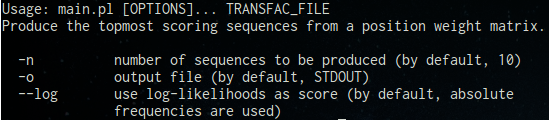
\includegraphics[scale=0.5]{perl}

%%%% EFFICACY %%%%

\subsection{Efficiency of the algorithm} \label{efficiency}
<<<<<<< HEAD

After an analysis of the algorithm and some mathematics, I have concluded that the time complexity of the algorithm is as follows:\\

Best case, with respect to \emph{l}: \ \ \ $\mathcal{O}(l)$

Best case, with respect to \emph{n}: \ \ $\mathcal{O}(n)$

Worst case, with respect to \emph{l}: \ $\mathcal{O}(l)$

=======

After an analysis of the algorithm and some mathematics, I have concluded that the time complexity of the algorithm is as follows:\\

Best case, with respect to \emph{l}: \ \ \ $\mathcal{O}(l)$

Best case, with respect to \emph{n}: \ \ $\mathcal{O}(n)$

Worst case, with respect to \emph{l}: \ $\mathcal{O}(l)$

>>>>>>> 94542c197c0712e0dd951ffb05a11457be670649
Worst case, with respect to \emph{n}: $\mathcal{O}(n^2)$

\section{Results} \label{results}

\subsection{Motif 1}

In the first case we have a very simple matrix, with zeros at many positions. We can easily see that the highest scoring position must be \emph{GGACATGCCCGGGCATGTCC}, with only a tie in the last position, which can either be a \emph{C} or a \emph{T}. Running this program we should obtain that sequence as the first one (due to the stable sorting of each position), and the same sequence with \emph{T} at the last position as the second one. Running the program to produce only the first ten sequences gives us the following results (in green, the nucleotides which don't vary across the ten sequences, in red, nucleotides which vary in at least two sequences):\\\\
\emph{./main.pl motif1.tf -n 10}
\begin{center}
\re{GG}\g{ACATG}C\g{CCGGGCATGT}C\re{C}\spaces307\\
\re{GG}\g{ACATG}C\g{CCGGGCATGT}C\re{T}\spaces307\\
\re{GG}\g{ACATG}C\g{CCGGGCATGT}C\re{G}\spaces302\\
\re{GA}\g{ACATG}C\g{CCGGGCATGT}C\re{C}\spaces300\\
\re{GA}\g{ACATG}C\g{CCGGGCATGT}C\re{T}\spaces300\\
\re{GG}\g{ACATG}C\g{CCGGGCATGT}C\re{A}\spaces300\\
\re{AG}\g{ACATG}C\g{CCGGGCATGT}C\re{C}\spaces298\\
\re{GG}\g{ACATG}T\g{CCGGGCATGT}C\re{C}\spaces298\\
\re{GG}\g{ACATG}C\g{CCGGGCATGT}T\re{C}\spaces298\\
\re{AG}\g{ACATG}C\g{CCGGGCATGT}C\re{T}\spaces298\\
\end{center}

The results conform to our expectations. There are two sequences with the highest possible score (which match perfectly the consensus letters of the \emph{transfac} file), and we can see that the next sequences are mainly variations of the first ones in the last, second, and first positions. This is logical, as this positions are, in that order, the ones which show a smallest difference of frequency among the most frequent nucleotide and the second one. We can also see that the sequences are ordered by score. This is due to the algorithm, which produces only the top-scoring sequences in an ordered fashion (the sequences are not sorted at any moment).
\subsection{Motif 2}
The results from the second motif are the following. In green, the nucleotides which don't vary. In red, those which vary in at least two sequences:\\\\
\emph{./main.pl motif2.tf -n 10}
\begin{center}

\re{ \g{AAT}T\g{TTCACGC}A\g{TGA}G\g{TT}\bl{C}\g{A}C } \spaces591\\
\re{ \g{AAT}T\g{TTCACGC}A\g{TGA}A\g{TT}\bl{C}\g{A}C } \spaces590\\
\re{ \g{AAT}C\g{TTCACGC}A\g{TGA}G\g{TT}\bl{C}\g{A}C } \spaces589\\
\re{ \g{AAT}T\g{TTCACGC}T\g{TGA}G\g{TT}\bl{C}\g{A}C } \spaces589\\
\re{ \g{AAT}T\g{TTCACGC}A\g{TGA}G\g{TT}\bl{C}\g{A}T } \spaces588\\
\re{ \g{AAT}C\g{TTCACGC}A\g{TGA}A\g{TT}\bl{C}\g{A}C } \spaces588\\
\re{ \g{AAT}T\g{TTCACGC}T\g{TGA}A\g{TT}\bl{C}\g{A}C } \spaces588\\
\re{ \g{AAT}T\g{TTCACGC}A\g{TGA}G\g{TT}\bl{A}\g{A}C } \spaces587\\
\re{ \g{AAT}T\g{TTCACGC}A\g{TGA}C\g{TT}\bl{C}\g{A}C } \spaces587\\
\re{ \g{AAT}T\g{TTCACGC}A\g{TGA}A\g{TT}\bl{C}\g{A}T } \spaces587\\

\end{center}

Again the results are logical: our sequences are correctly ordered and each sequence is a variation in one single nucleotide of one of the previous sequences. The positions in red vary more due to the fact that the difference among the most frequent nucleotide and the second most frequent in that position is smaller, which makes it easier to change it maintaining a hight score.

\end{document}
